
\chapter{Data on the Sphere}
\label{ch_intro}

\section{Introduction}

In a number of areas of scientific activity, data is gathered which naturally maps to the sphere. For instance, remote sensing of the 
Earth's surface and atmosphere,\emph{e.g.} with POLDER\footnote{\emph{http://polder.cnes.fr}}, generates spherical data maps which are 
crucial for global and local geophysical studies such as understanding climate change, geodynamics or monitoring human-environment 
interactions. More examples can be found in medical imaging or computer graphics. In astronomy and astrophysics, recent and upcoming 
ground based and satellite borne experiments such as WMAP\footnote{\emph{http://map.gsfc.nasa.gov}} or Planck-Surveyor\footnote{\emph{http://astro.estec.esa.nl/Planck}} 
for the observation of the Cosmic Microwave Background radiation field over the whole celestial sphere, have and will produce full-sky 
maps in a wide range of wavelengths. These maps are necessarily digitized and hence distributed as a finite set of pixel values on some 
grid. The properties of this grid will affect the subsequent analysis of the data, and a good choice will make standard computations, 
such as the spherical harmonics transform, much faster and accurate. Considerable work has been dedicated to the development of 
pixelization schemes on the sphere. In particular, Healpix\cite{healpix} is a sampling scheme which has some attractive geometrical 
features profitably used in this spherical data analysis software package. \\

Processing spherical data maps requires specific tools or somehow adapting traditional methods used on flat images to the spherical 
topology, such as multiscale transforms for image processing. Among these, Wavelets and related representations are by now successfully 
used in all areas of signal and image processing. Their recent inclusion in JPEG 2000 -- the new still-picture compression standard -- 
is an illustration of this lasting and significant impact. Wavelets are also very popular tools in astronomy \cite{starck:book02} which 
have led to very impressive results in denoising and detection applications. For instance, both the Chandra and the XMM data centers 
use wavelets for the detection of extended sources in X-ray images. For denoising and deconvolution, wavelets have also demonstrated 
how powerful they are for discriminating signal from noise \cite{starck:sta02_2}. In cosmology, wavelets have been used in many studies 
such as for analyzing the spatial distribution of galaxies \cite{astro:slezak93,astro:escalera95,starck:sta05,starck:martinez05}, 
determining the topology of the universe \cite{astro:rocha04}, detecting non-Gaussianity in the CMB maps \cite{gauss:aghanim99,gauss:barreiro01_1,wave:vielva04,starck:sta03_1},
reconstructing the primordial power spectrum \cite{astro:pia03}, measuring the galaxy power spectrum \cite{astro:fang00} or reconstructing 
weak lensing mass maps \cite{starck:sta05b}. It has also been shown that noise is a problem of major concern for N-body simulations of 
structure formation in the early Universe and that using wavelets for removing noise from N-body simulations is equivalent to simulations 
with two orders of magnitude more particles \cite{rest:romeo03,rest:romeo04}. 

Wavelets owe part of their success to their ability for sparse approximation of point singularities. However they are not as good at detecting 
highly anisotropic features such as curvilinear singularities in images. This is where other multiscale systems such as Ridgelets \cite{cur:candes99_1} 
and Curvelets \cite{cur:donoho99,starck:sta01_3}, which exhibit high directional sensitivity and are highly anisotropic, come into play. Digital 
implementations of both ridgelet and curvelet transforms for image denoising are described in \cite{starck:sta01_3}. Inspired by the successes 
of \emph{Euclidean} wavelets, ridgelets and curvelets, this package provides implementations of new multiscale decompositions for spherical images 
namely the isotropic undecimated wavelet transform, the ridgelet transform and the curvelet transform each of which is invertible.

\section{Pixelization}

Despite the apparent simplicity of the sphere, deriving numerical schemes on the sphere is not a trivial task. A major difficulty encountered 
in the design of numerical methods on the sphere is that of pixelization: there is no obvious way in which to reconcile the requirements 
for a \emph{maximally} uniform sampling and for an exact and invertible computation of the spherical harmonics decomposition of band-limited 
functions \cite{healpix,icosahedron}. Also, the sampling strategy determines largely the achievable algorithmic complexity of these computations. 
Several sampling schemes have been proposed recently such as Tegmark's Icosahedron \cite{icosahedron}, the Igloo \cite{igloo} or Healpix \cite{healpix} 
methods which tend to favor approximate uniformity among other properties. The Glesp \cite{glesp} pixelization was developed with a strong 
focus on the accuracy of the spherical harmonics transform. 

\subsection*{Healpix}

The Healpix representation is a curvilinear hierarchical partition of the sphere into quadrilateral pixels of exactly equal area but with 
varying shape. The base resolution divides the sphere into 12 quadrilateral faces of equal area placed on three rings around the poles 
and equator. Each face is subsequently divided into $nside^{2}$ pixels following a quadrilateral multiscale tree structure. The pixel 
centers are located on iso-latitude rings, and pixels from the same ring are equispaced in azimuth. This is critical for computational 
speed of all operations involving the evaluation of spherical harmonics transforms, including standard numerical analysis operations such 
as convolutions, power spectrum estimation\ldots \\

\begin{figure}
\centering
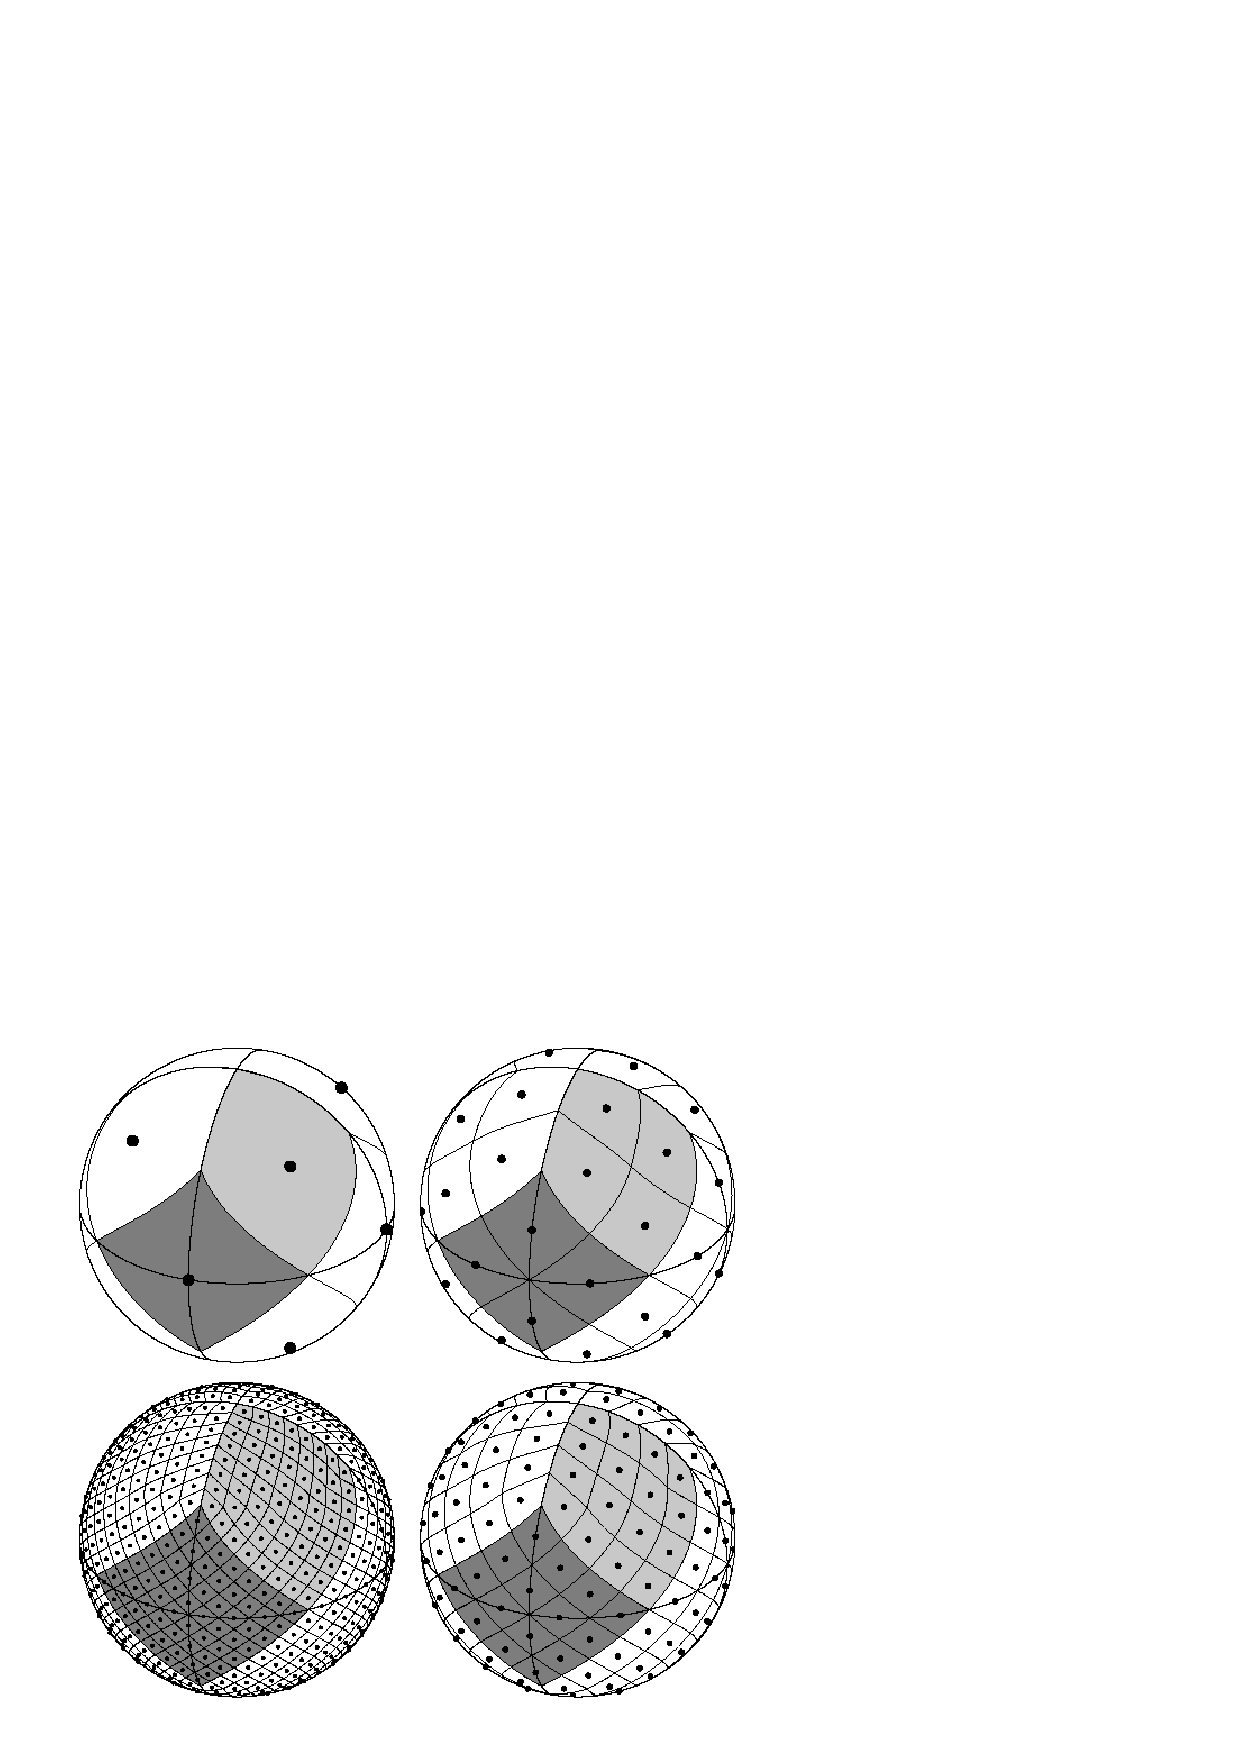
\includegraphics{pixelhealpix}
\caption{The Healpix sampling grid.}
\label{pixelhealpix}
\end{figure}

An important geometrical feature of the Healpix sampling grid is the hierarchical quadrilateral tree structure. This defines a \emph{natural} 
one-to-one mapping of the sphere sampled according to the Healpix grid, into twelve \emph{flat} images, on all scales. It is then easy to 
partition a spherical map using Healpix into quadrilateral blocks of a specified size. One first extracts the twelve base-resolution faces, 
and each face is then decomposed into overlapping blocks of the specified size. This decomposition into blocks is an essential step of the 
traditional \emph{flat} 2D curvelet transform. Based on the reversible warping of the sphere into a set of flat images made possible by the 
Healpix sampling grid, the ridgelet and curvelet transforms can be extended to the sphere. 

With the decomposition into blocks described above, there is no overlapping between neighboring blocks belonging to different base-resolution faces. 
This may result for instance in blocking effects in denoising experiments \emph{via} non linear filtering. It is possible to overcome this difficulty 
in some sense by working simultaneously with various rotations of the data with respect to the sampling grid. This will average out undesirable 
effects at edges between base resolution faces. 

\section{Multiscale methods on the sphere}

\subsection{Wavelets on the sphere}

In the last years, several wavelet transforms on the sphere have been proposed. Schr{\"o}der and Sweldens \cite{wave:sweldens95a} have developed 
an orthogonal wavelet transform on the sphere based on the Haar wavelet function which then suffers from the poor properties of the Haar function 
and the problems inherent to the orthogonal decomposition. A few papers describe continuous wavelet transforms on the sphere \cite{wave:antoine99,wave:tenerio99,wave:cayon01,wave:holschneider96}. 
An application to the detection of non-Gaussianity in the CMB radiation using the stereographic Mexican hat wavelet is reported in \cite{wave:vielva04}. 
These methods have been extended to directional wavelet transforms \cite{wave:antoine01,wave:hobson04,wave:wiaux}. Although profitable for data 
analysis, these continuous transforms lack an inverse transform and hence are clearly not suitable for restoration purposes. The algorithm proposed 
by Freeden and Maier\cite{freeden97,freeden98}, based on the Spherical Harmonic Decomposition, is to our knowledge the only one to have an inverse transform.\\  

A very popular wavelet algorithm in astrophysical applications is the so-called ``\emph{\`a trous} algorithm'' (a better name would be the 
``isotropic undecimated wavelet transform'' ), which possesses the following features: i) it is isotropic, ii) it is undecimated, iii) it uses 
an order three Box-Spline as scaling function. The isotropy of the wavelet function makes this decomposition optimal for the detection of 
isotropic objects. The non decimation makes the decomposition redundant (the number of coefficients in the decomposition is equal to the number 
of samples in the data multiplied by the number of scales) and allows us to avoid Gibbs aliasing after reconstruction in image restoration 
applications, as generally occurs with orthogonal or bi-orthogonal wavelet transforms. The choice of a $B_3$-spline is motivated by the fact 
that we want an analyzing function close to a Gaussian, but verifying the dilation equation, which is required in order to have a fast transformation. 
Finally the last property of this algorithm is to provide a very straightforward reconstruction. Indeed, the sum of all the wavelet scales and 
of the coarsest resolution image reproduces exactly the original image. \\

The \mrs package offers an implementation of a new isotropic wavelet transform on the sphere. Its properties are similar to those of the \emph{\`a trous} 
algorithm and therefore should be very useful for data denoising and deconvolution. This algorithm, described in chapter~\ref{ch_mms}, is directly derived
from the FFT-based wavelet transform proposed in\cite{starck:sta94_3} for aperture synthesis image restoration. It is relatively close to the Freeden and 
Maier \cite{freeden98} method, except that the reconstruction process is as straightforward as in the \emph{\`a trous} algorithm (i.e. the sum of the scales 
reproduces the original data). This new wavelet transform can also be easily extended to a pyramidal wavelet transform, which may be very important for 
larger data sets such such as from the future Planck experiment.

\subsection{Ridgelets and Curvelets on the sphere}
 
When analyzing data which contains anisotropic features, wavelets are no longer optimal. This has motivated the development of new multiscale 
decompositions such as the ridgelet and the curvelet transforms \cite{cur:donoho99,starck:sta01_3}. Among possible applications of those data 
analysis methods, it was shown in Starck et al. \cite*{starck:sta03_1} that the \emph{flat} curvelet transform could be useful for the detection 
of non Gaussianity in \emph{flat} patches of CMB data, and also to discriminate among different causes of non Gaussianity. 

In this area, further insight will come from the analysis of full-sky data mapped to the sphere thus requiring the development of a curvelet 
transform on the sphere. The \mrs package offers an implementation of ridgelet and curvelet transforms for spherical maps. Those implementations 
are derived as extensions of the digital ridgelet and curvelet transforms described in \cite{starck:sta01_3}. The implemented undecimated isotropic 
wavelet transform on the sphere and the specific geometry of the Healpix sampling grid are important components of the present implementation of 
curvelets on the sphere. \\
 
Further motivation for developing these new multiscale methods on the sphere follows from the results obtained in different data processing applications. 
As described in chapter\ref{ch_restore}, the \mrs package provides the necessary tools to experiment with these new spherical multiscale transforms in 
denoising applications, for instance using the Combined Filtering Method, which allows us to filter data on the sphere using both the Wavelet and the 
Curvelet transforms. The analysis of multichannel data mapped to the sphere, a problem encountered for instance in the processing of WMAP and Planck 
observations, is another issue that is shown to benefit from the developed multiscale representations on the sphere. This is reported in chapter~\ref{ch_mrs_ica} 
which is dedicated to describing some methods in multichannel data analysis extended to spherical maps which are implemented in the \mrs package.  
 
\section{Processing of polarized datas on the sphere}

Polarized maps are a special kind of multi-dimentionnal datas with strong links between their components. The polarization is of great importance 
in physics or astrophysics as it's analysis denotes fundamentals characteristics of the observed object or phenomenum. An example of great interest 
is today the cosmic microwave background \cite{starck}.

The statistical analysis of the slight intensity fluctuations in the primordial cosmic microwave background radiation field, for which evidence was 
found for the first time in the early 1990's in the observations made by COBE~\cite{gauss:smoot92}, is a major issue in modern cosmology as these 
are strongly related to the cosmological scenarios describing the properties and evolution of our Universe. In the Big Bang model, the observed CMB 
anisotropies are an imprint of primordial fluctuations in baryon-photon density from a time when the temperature of the Universe was high enough above 
3000~K for matter and radiation to be tightly coupled. At that time, the attraction of gravity and the repulsive radiation pressure were opposed, thus 
generating so-called acoustic oscillations in the baryon-photon fluid, causing peaks and troughs to appear in the power spectrum of the spatial anisotropies 
of the CMB. With the Universe cooling down as it expanded, matter and radiation finally decoupled. Photons were set free in a nearly transparent Universe, 
while the density fluctuations collapsed under the effect of gravity into large scale structures such as galaxies or clusters of galaxies. Due to the 
expansion of the Universe, the CMB photons are now observed in the microwave range but are still distributed according to an almost perfect black body 
emission law. Another major result was the measurement of the polarization state and anisotropies of the CMB radiation field by DASI~\cite{dasi}. 
Only a fraction of the total CMB radiation is polarized so that extremely sensitive instruments are needed. Polarization of the CMB radiation is a 
consequence of the Thomson scattering of photons on electrons. But for the outgoing population of photons to be polarized, the radiation incident on 
the scatterer needs to be anisotropic and have a quadrupole moment. The statistics of the CMB polarization anisotropies are also a source of information 
for cosmology. Inference of cosmological parameters from the joint statistics of the CMB anisotropies should benefit from both the complementarity and 
the redundancy of the information carried by the additional measurement of CMB polarization. Hence the full-sky maps with unprecedented sensitivity and 
angular resolution of both temperature and polarization anisotropies of the CMB to be delivered by the upcoming Planck Surveyor satellite experiment are 
awaited with excitement.

\subsection{Orthogonal representation of polarized datas}
\label{sec:polar}

\begin{figure*}[htb]
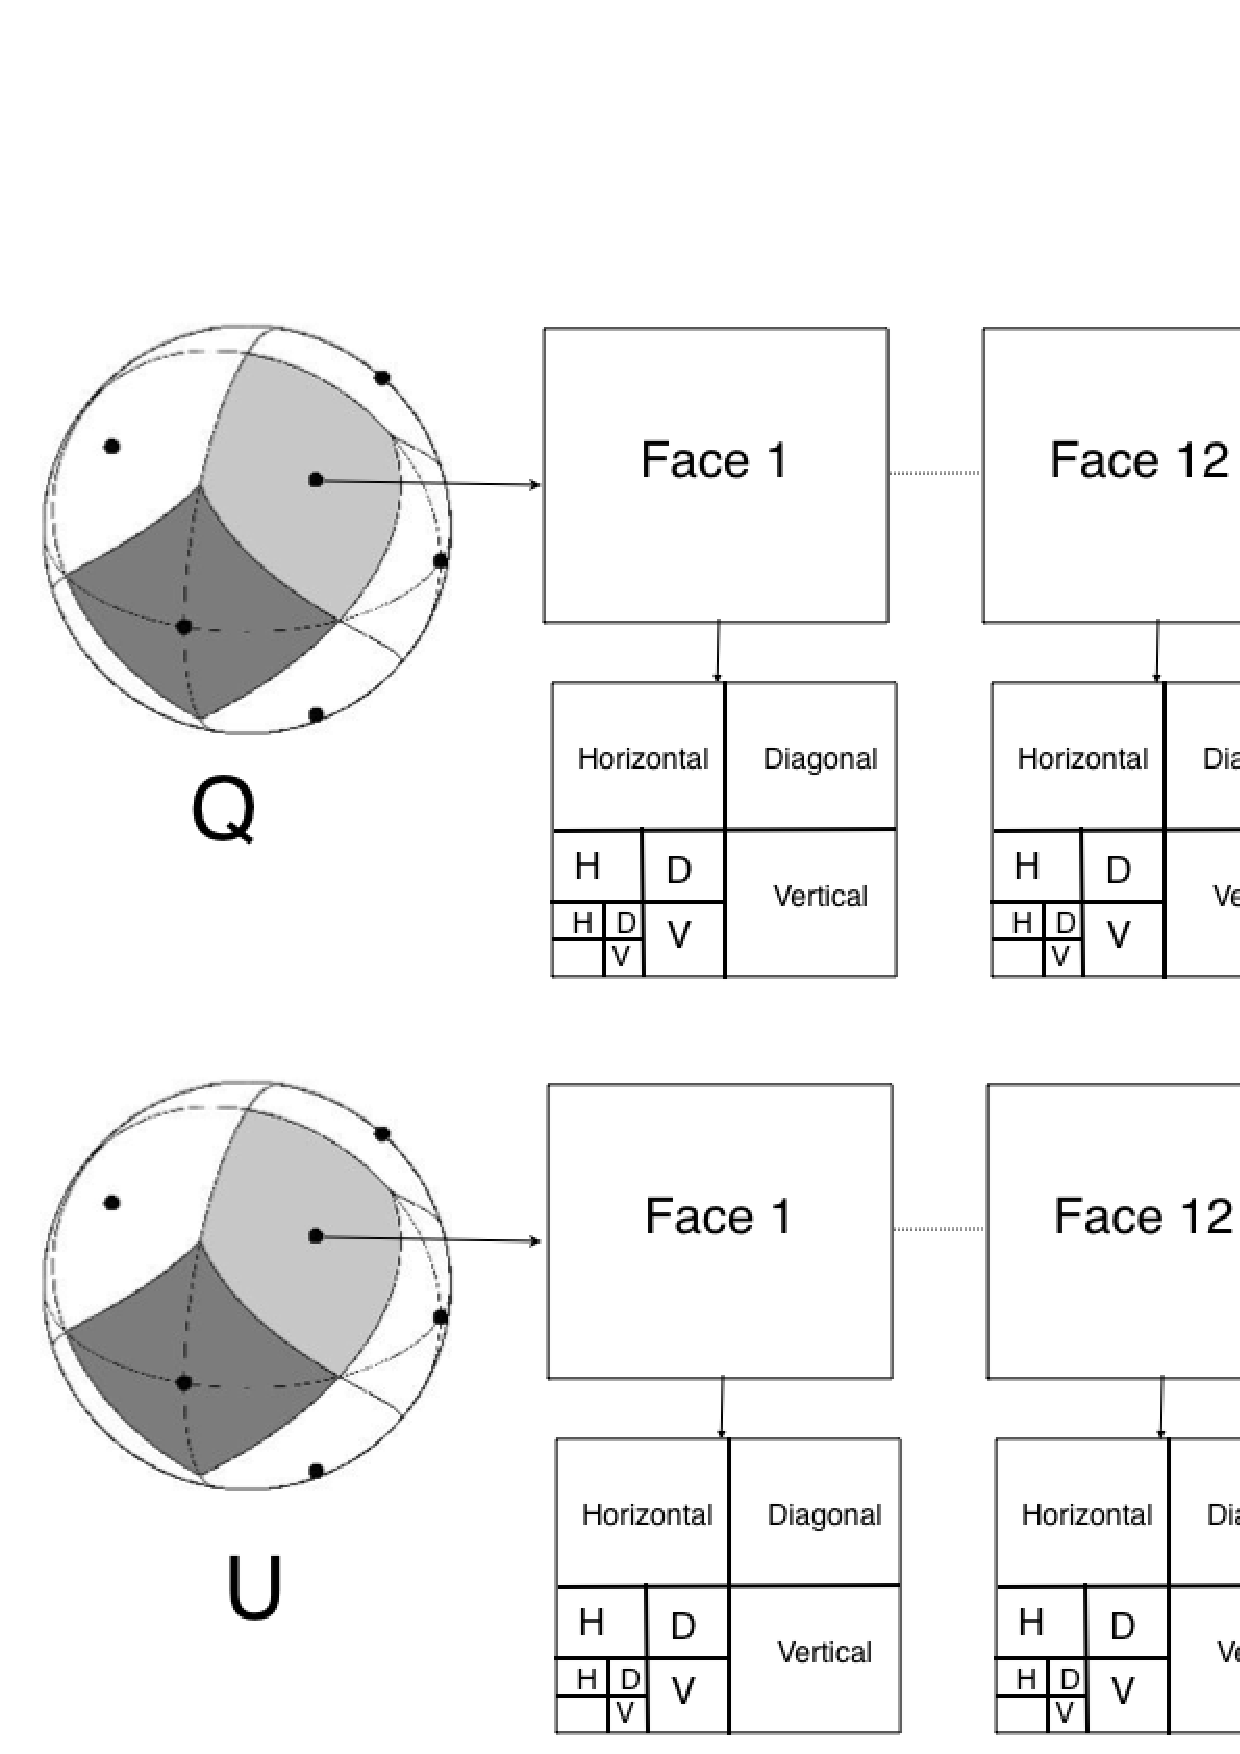
\includegraphics[width=\textwidth]{fig_pola_qu_owt_trans.pdf}
\caption{Q-U orthogonal Wavelet Transform.}
\label{fig_qu_owt_trans}
\end{figure*}
Full-sky CMB polarization data, as expected from the upcoming Planck experiment, consists of measurements of the Stokes parameters so that in addition 
to the temperature $T$ map, $Q$ and $U$ maps are given as well. The fourth Stokes parameter commonly denoted $V$ is a measure of circular polarization. 
In the case of CMB which is not expected to have circularly polarized anisotropies, $V$ vanishes. The former three quantities, $T$, $Q$ and $U$ then 
fully describe the linear polarization state of the CMB radiation incident along some radial line of sight : $T$ is the total incoming intensity, $Q$ is 
the difference between the intensities transmitted by two perfect orthogonal polarizers the directions of which define a reference frame in the tangent 
plane, and $U$ is the same as $Q$ but with polarizers rotated 45 degrees in that tangent plane. Clearly, $Q$ and $U$ are not invariant through a rotation 
of angle $\phi$ of the local reference frame around the line of sight. In fact, it is easily shown that~:
\begin{eqnarray}
Q ' = & \cos (2 \phi) Q + \sin(2 \phi) U \\ \nonumber
U ' = & \cos (2 \phi) U - \sin(2 \phi) Q 
\end{eqnarray}
which can also be written $Q' \pm i U' = e^{\mp i\phi} ( Q \pm i U )$ which by definition expresses the fact that the quantities $Q \pm i U$ are 
spin-2 fields on the sphere. The suitable generalization of the Fourier representation for such fields is the spin-2 spherical harmonics basis 
denoted $_{\pm 2}Y_{\ell m}$, in which we can expand~: 
\begin{eqnarray}\label{QU}
Q \pm i U  = \sum_{\ell, m} { _{\pm 2}a_{\ell m}} {_{\pm 2}Y_{\ell m} }
\end{eqnarray}

It is convenient~\cite{zalda} to introduce the two quantities denoted $E$ and $B$ which are defined on the sphere by~:
\begin{eqnarray}\label{EB}
E = & \sum_{\ell, m} a_{\ell m} ^E Y_{\ell m} = \sum_{\ell, m} - \frac{1}{2} ( {_{ 2}a_{\ell m}} + {_{- 2}a_{\ell m}} ) Y_{\ell m} \\ \nonumber
B = & \sum_{\ell, m} a_{\ell m} ^B Y_{\ell m} = \sum_{\ell, m} i \frac{1}{2} ( {_{ 2}a_{\ell m}} - {_{- 2}a_{\ell m}} ) Y_{\ell m} 
\end{eqnarray}

\subsection{Multiscale transform on the sphere for polarized datas}

Inprovements in the second version of the \mrs package includes extension of the 1D multiscale transforms to the case of polarized maps with 
the three fields $T$, $Q$ and $U$ (or the fields $T$, $E$ and $B$). The easiest way to build a multiscale transform for polarized data is to 
use the Healpix\footnote{http://healpix.jpl.nasa.gov} representation \cite{pixel:healpix}, and to apply a bi-orthogonal wavelet transform 
on each face of the Healpix map, separately for $Q$ and $U$. Fig.~\ref{fig_qu_owt_trans} shows the flow-graph of this Q-U orthogonal wavelet 
transform (QU-OWT). Most of the algorithms included in \mrs for the processing of 1D images know have a version for polarized maps.

% \clearpage
% \newpage
